\subsection{RemotePeerMeter}\label{sec:mit-peer-meter}
Based on the \lstinline|RemotePeerMeter| the \lstinline|PeerManager| gathers information about the quality of a \lstinline|RemotePeer|. The quality of a peer is needed for finding the optimal routing path for messages and finding new connection candidates.
Besides the quality, the RemotePeerMeter also provides other metrics that are presented in \vref{fig:mit-remote-peer-meter} and further described in the following paragraphs.

\begin{figure}
\centering
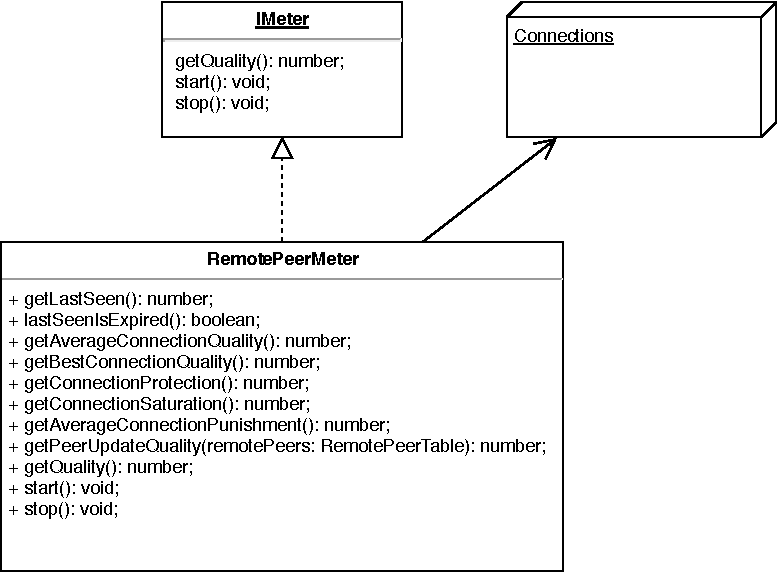
\includegraphics[width=0.75\textwidth]{graphics/implementation/mitosis-architecture-PeerMeter.pdf}
\caption{RemotePeerMeter}
\label{fig:mit-remote-peer-meter}
\end{figure}

\paragraph{LastSeen}
\lstinline|LastSeen| is a metric that represents the vitality of a peer. Each time a message is received from a RemotePeer its LastSeen timestamp is set to the current tick. The longer a RemotePeer has not send a message the older its LastSeen gets. When it exceeds a certain threshold, the RemotePeer is assumed to have crashed and is consequently removed.
As a remote peer can have multiple connections the LastSeen metric is based on the youngest LastSeen of all connections (\vref{lst:mit-last-seen}). Youngest means a more recent LastSeen.

Whether the peer is seen as crashed is determined by the delta value of the current application tick and the youngest last seen (\vref{lst:mit-crashed}).

\paragraph{Connection Quality}
The connection is responsible for measuring its quality to a RemotePeer. Each connection type has its own mechanism to do so. This is further explained in \vref{sec:mit-connections}.
The RemotePeerMeter can determine the average connection quality (\vref{lst:mit-average-connection-quality}) and the best available connection quality (\vref{lst:mit-best-connection-quality}).

\paragraph{RemotePeer Newcomer Protection}
When a connection to a new RemotePeer is established the \textit{Newcomer Protection} is activated as long as the new peer does not have any other connections. This prevents that the new RemotePeer might be kicked out immediately because of the peer's desire to reach its own connection goal. The Newcomer Protection is active for a globally defined time window, but ends if the other peer has managed to establish connections to other peers (\vref{lst:mit-welpenschutz}).

\paragraph{Connection Saturation}
The connection saturation of a RemotePeer is calculated by counting all reported connections and the amount of direction connections. Each peer has the desire to obtain a certain number of RemotePeers (the default is $\ 5 $). Additionally, peers are required to stay below a maximum limit of allowed connections (the default is $\ 10 $). This applies to all peers, therefore a peer can derive how many free connections a remote peer has. \vref{fig:mit-remote-peer-saturation} shows a sample calculation and \vref{lst:mit-connection-saturation} the corresponding pseudo code. 
However, this is just an estimation because a peer only knows the reports of direct peers. As seen in the \vref{fig:mit-remote-peer-saturation} \textit{Node D} is also connected to \textit{Node E}, but as \textit{Node A} does not have a direct connection to \textit{Node E}, it does not know about its existence.
The saturation estimation is limited to a value between $\ 0 $ and $\ 1 $. As long as the estimated connection count is below the minimum connection goal, the value is $\ 0 $, otherwise in the range between $\ 0 $ and $\ 1 $, where $\ 0 $ is a good probability and $\ 1 $ a bad one.
The saturation value is used when alternative RemotePeers are recommended to a peer, that is trying to connect but the maximum connection limit is already reached.

\begin{figure}
\centering
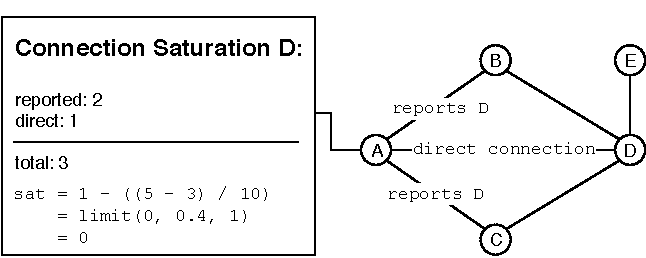
\includegraphics[width=0.75\textwidth]{graphics/implementation/mitosis-architecture-Connection-Saturation.pdf}
\caption{Peer A's calculation of RemotePeer D's Saturation }
\label{fig:mit-remote-peer-saturation}
\end{figure}

\paragraph{Connection Punishment}
A punishment for a connection is applied when it can not be successfully established within a globally defined time window or is prematurely closed. The punishment shall ensure that the peer does not immediately retry to open a connection. After a cool–off phase the punishment for a connection is revoked.
The RemotePeerMeter provides the metric of the average amount of punished connections. When a peer has a lot of punished connections it is less likely considered in the peer selection.

\paragraph{Report Quality}\label{par:mit-report-quality}
A peer is reporting its direct neighbours via a \peerUpdate, where each RemotePeer has a quality. The quality is calculated by the best connection quality to a given remote peer and its connection saturation (\vref{lst:mit-remote-peer-quality-report}). Based on the reported quality in the \peerUpdate, the receiver can select the RemotePeer as a potential connection partner. 

\paragraph{RemotePeer Quality}
The RemotePeer quality is used during the selection process of the PeerManager for message delivery. The quality is derived by the average connection quality and a punishment factor (\vref{lst:mit-remote-peer-quality}). When a peer has a lot of punished connections it is considered unstable and is selected less likely for message delivery.

\paragraph{Router Link Quality}
Each RemotePeer is maintaining a router link quality, meaning that a peer who receives a router alive first ranks higher than one that receives it later. A router alive messages contains a sequence number. When the sequence number is unknown, the PeerManager adds a new sequence with an undefined rank for all directly connected RemotePeers. Afterwards the rank of the RemotePeer who has delivered the message is set to $\ 1 $.
When a router alive message is received with a sequence number that is already known, the rank of the delivering peer is set to the amount of RemotePeers who have delivered it already.
The link quality is an average of the rank of all received sequence numbers. When a sequence number does not have a rank it is ignored.
The goal of the router link quality is to bring peers closer to the router. During the peer selection process, RemotePeers connected to a direct neighbour with a high link quality are favoured.
